\documentclass[final]{beamer}

\usepackage[scale=1.24]{beamerposter} % Use the beamerposter package for laying out the poster

\usetheme{confposter} % Use the confposter theme supplied with this template

\setbeamercolor{block title}{fg=nblue,bg=white} % Colors of the block titles
\setbeamercolor{block body}{fg=black,bg=white} % Colors of the body of blocks
\setbeamercolor{block alerted title}{fg=white,bg=dblue!70} % Colors of the highlighted block titles
\setbeamercolor{block alerted body}{fg=black,bg=dblue!10} % Colors of the body of highlighted blocks
% Many more colors are available for use in beamerthemeconfposter.sty

\newlength{\sepwid}
\newlength{\colonewid}
\newlength{\coltwowid}
\newlength{\onecolwid}
\setlength{\paperwidth}{48in} % A0 width: 46.8in
\setlength{\paperheight}{36in} % A0 height: 33.1in
\setlength{\sepwid}{0.024\paperwidth} % Separation width (white space) between columns
\setlength{\onecolwid}{0.301\paperwidth} % Width of one column
\setlength{\colonewid}{0.27\paperwidth} % Width of column one
\setlength{\coltwowid}{0.28\paperwidth} % Width of column two
\setlength{\topmargin}{-0.5in} % Reduce the top margin size
% -----------------------------------------------------------

\usepackage{graphicx}  % Required for including images
\usepackage{booktabs} % Top and bottom rules for tables
\usepackage{tikz}
\usetikzlibrary{
  arrows,
  calc,
  decorations.pathmorphing,
  decorations.pathreplacing,
  decorations.markings,
  fadings,
  positioning,
  shapes,
  arrows.meta
}
\usepgfmodule{oo}

\pgfdeclareradialshading{glow2}{\pgfpoint{0cm}{0cm}}{
  color(0mm)=(white);
  color(2mm)=(white);
  color(8mm)=(black);
  color(10mm)=(black)
}
\pgfdeclareradialshading{glow}{\pgfpoint{0cm}{0cm}}{
  color(0mm)=(white);
  color(5mm)=(white);
  color(9mm)=(black);
  color(10mm)=(black)
}

\begin{tikzfadingfrompicture}[name=glow fading]
  \shade [shading=glow] (0,0) circle (1);
\end{tikzfadingfrompicture}

\begin{tikzfadingfrompicture}[name=glow2 fading]
  \shade [shading=glow2] (0,0) circle (1);
\end{tikzfadingfrompicture}

\pgfdeclarelayer{tweezer}
\pgfsetlayers{tweezer,main}
\pgfooclass{tweezer}{
  \method tweezer() {
  }
  \method drawTweezer(#1,#2,#3) {
    \begin{pgfonlayer}{tweezer}
      \shade[shading=radial,path fading=glow fading,shift={(#1,#2)},rotate=90,yscale=1,
      fill opacity=0.9,inner color=#3]
      plot[draw,samples=200,domain=-1.5:1.5] function {sqrt(0.01 + x**2 / 5)}
      -- plot[draw,samples=200,domain=1.5:-1.5] function {-sqrt(0.01 + x**2 / 5)};
    \end{pgfonlayer}
  }
  \method drawAtom(#1,#2,#3,#4) {
    \fill [#4,path fading=glow2 fading] (#1,#2) circle (#3);
  }
  \method drawNaAtom(#1,#2,#3) {
    \pgfoothis.drawAtom(#1,#2,#3,orange);
  }
  \method drawCsAtom(#1,#2,#3) {
    \pgfoothis.drawAtom(#1,#2,#3,blue);
  }
  \method drawNaTweezer(#1,#2) {
    \pgfoothis.drawTweezer(#1,#2,orange!35!black!30);
  }
  \method drawCsTweezer(#1,#2) {
    \pgfoothis.drawTweezer(#1,#2,blue!30!black!30);
  }
  \method up(#1,#2) {
    \pgfoothis.drawCsTweezer(#1,#2);
    \pgfoothis.drawNaAtom(#1,#2+0.06,0.12);
    \pgfoothis.drawCsAtom(#1,#2-0.06,0.16);
  }
  \method down(#1,#2) {
    \pgfoothis.drawCsTweezer(#1,#2);
    \pgfoothis.drawCsAtom(#1,#2+0.06,0.16);
    \pgfoothis.drawNaAtom(#1,#2-0.06,0.12);
  }
  \method naTrap(#1,#2) {
    \pgfoothis.drawNaTweezer(#1,#2);
    \pgfoothis.drawNaAtom(#1,#2,0.12);
  }
  \method csTrap(#1,#2) {
    \pgfoothis.drawCsTweezer(#1,#2);
    \pgfoothis.drawCsAtom(#1,#2,0.16);
  }
}
\pgfoonew \mytweezer=new tweezer()

% ----------------------------------------------------------------------------------------
%	TITLE SECTION
% ----------------------------------------------------------------------------------------

\def\realtitle{Association of single ultracold molecules in optical tweezers}

\title{%
  \texorpdfstring{%
    \makebox[\linewidth]{%
      \makebox[0pt][l]{%
        \raisebox{\dimexpr-\height+\baselineskip}[0pt][0pt]
        {
\includegraphics[height=4\baselineskip]{harvard}}% Left logo
      }\hfill
      \makebox[0pt]{\textcolor{dblue}{\realtitle}}%
      \hfill\makebox[0pt][r]{%
        \raisebox{\dimexpr-\height+0.5\baselineskip}[0pt][0pt]
        {
\includegraphics[height=3\baselineskip]{cua}}% Right logo
      }%
    }%
  }
  {\realtitle}} % Poster title

\author{Yichao Yu, Jonathan Hood, Lee R. Liu, Jessie T. Zhang, Yen-Wei Lin,
  Kenneth Wang, Rem\'y Vatr\'e, Till Rosenband, Kang-Kuen Ni}
\institute{Harvard-MIT Center for Ultracold Atoms\\
  Department of Chemistry and Chemical Biology and Department of Physics, Harvard University}

% ----------------------------------------------------------------------------------------

\begin{document}

\addtobeamertemplate{block end}{}{\vspace*{2ex}} % White space under blocks
\addtobeamertemplate{block alerted end}{}{\vspace*{2ex}} % White space under highlighted (alert) blocks

\setlength{\belowcaptionskip}{2ex} % White space under figures
\setlength\belowdisplayshortskip{2ex} % White space under equations

\begin{frame}[t] % The whole poster is enclosed in one beamer frame
  \begin{columns}[t]
    \begin{column}{\sepwid}\end{column} % Empty spacer column
    \begin{column}{\colonewid} % The first column
      \begin{block}{Ultracold Molecules}
        \begin{columns}[T]
          \begin{column}{0.57\colonewid}
            \vspace{3ex}
            \begin{itemize}
            \item NaCs has a large permanent electric dipole moment ($\mathbf{4.6}$ \textbf{Debye})
            \item Strong anisotropic dipole-dipole interactions
            \item Coupled internal degrees of freedom
              can be used to tune interactions and store information
            \end{itemize}
          \end{column}
          \begin{column}{0.42\colonewid}
            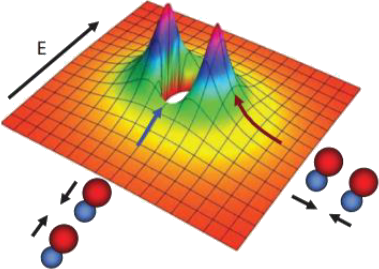
\includegraphics[width=0.4\colonewid]{reaction-align}
          \end{column}
        \end{columns}
        \begin{center}
          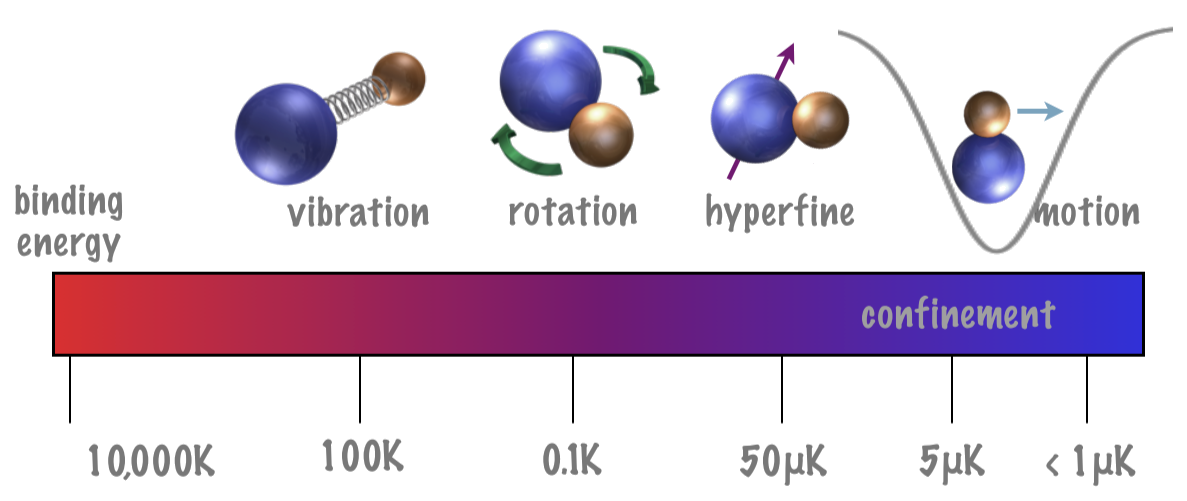
\includegraphics[width=0.8\colonewid]{temp-scale}
        \end{center}
      \end{block}

      \begin{block}{Our approach}
        \begin{columns}[T]
          \begin{column}{0.5\colonewid}
            \vspace{5ex}
            \begin{itemize}
            \item Assemble and trap individual molecules in optical tweezers
              from laser-cooled atoms
            \item Raman transition from atoms to weakly-bound molecules
            \item STIRAP to ground state molecules
            \end{itemize}
            \vspace{10ex}
            \textbf{\color{dblue}{Advantages}}
            \begin{itemize}
            \item Fast cycle time (<1s), small vacuum chamber
            \item Dynamically configurable trapping geometry
            \item All optical cooling and state-manipulation
            \end{itemize}
          \end{column}
          \begin{column}{0.44\colonewid}
            \begin{tikzpicture}[scale=2.5]
              \foreach \xoff in {0,2.2} {
                \mytweezer.drawCsTweezer(0+\xoff, -0.5)
                \mytweezer.drawNaTweezer(-1+\xoff, -0.5)
                \mytweezer.drawCsAtom(-0.07+\xoff, -0.42, 0.22)
                \mytweezer.drawNaAtom(-1.06+\xoff, -0.59, 0.27)

                \mytweezer.drawCsTweezer(0+\xoff, -3.1)
                \mytweezer.drawNaTweezer(-1+\xoff, -3.1)
                \mytweezer.drawCsAtom(0.0+\xoff, -3.1, 0.12)
                \mytweezer.drawNaAtom(-1.0+\xoff, -3.1, 0.16)

                \mytweezer.drawCsTweezer(-1+\xoff, -7.0)
                \mytweezer.drawNaAtom(-1.05+\xoff, -6.87, 0.16)
                \mytweezer.drawCsAtom(-0.95+\xoff, -7.13, 0.12)

                \mytweezer.drawCsTweezer(-1+\xoff, -9.5)
                \mytweezer.drawNaAtom(-1.02+\xoff, -9.44, 0.16)
                \mytweezer.drawCsAtom(-0.98+\xoff, -9.56, 0.12)

                \begin{scope}[opacity=0.4]
                  \draw[orange,loosely dotted,line width=5] (-1+\xoff, -0.9) -- (-1+\xoff, -2.9);
                  \draw[blue,loosely dotted,line width=5] (0+\xoff, -0.65) -- (0+\xoff, -2.9);
                  \draw[->,orange,line width=5] (-1+\xoff, -3.3) -- (-1+\xoff, -6.7);
                  \draw[->,blue,domain=-3.3:-6.7,smooth,variable=\y,line width=5]
                  plot ({atan((\y+4.7) * 5) / 170 - 0.5+\xoff},{\y});
                \end{scope}
                \draw[orange!50!blue,loosely dotted,line width=5,opacity=0.7]
                (-1+\xoff, -7.3) -- (-1+\xoff, -9.3);
              }
              \node[below,rotate=-90] at (3.3, -1.8) {Trapping and cooling};
              \node[below,rotate=-90] at (2.3, -7) {Merging};
              \node[below,rotate=-90,align=center] at (2.6, -9.5) {Forming\\molecules};
            \end{tikzpicture}
          \end{column}
        \end{columns}
      \end{block}

      \begin{block}{Acknowledgements}
        \begin{center}
          
\includegraphics[height=0.18\colonewid]{beckman}
          \hspace{15ex}
\includegraphics[height=0.18\colonewid]{nsf}\\
          
\includegraphics[height=0.18\colonewid]{afosr}
          \hspace{5ex}
\includegraphics[height=0.18\colonewid]{sloan}
        \end{center}
      \end{block}
    \end{column} % End of the first column

    \begin{column}{\sepwid}\end{column} % Empty spacer column

    \begin{column}{\coltwowid}
      \begin{block}{Trapping and cooling of atoms}
        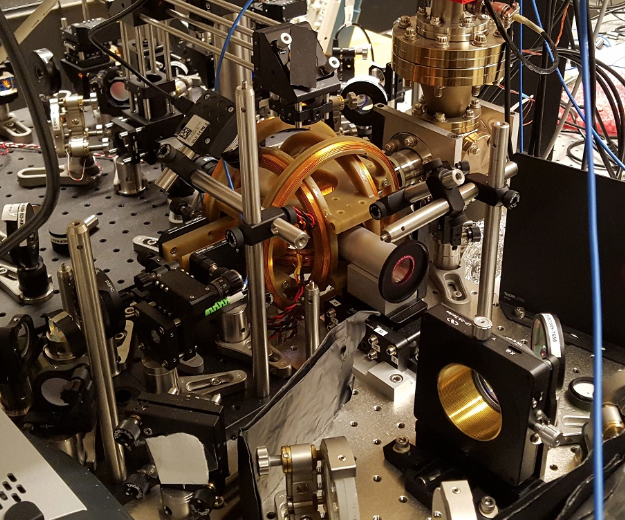
\includegraphics[width=0.5\coltwowid]{exp-photo}
      \end{block}
    \end{column} % End of the second column

    \begin{column}{\sepwid}\end{column} % Empty spacer column

    \begin{column}{\onecolwid} % The third column

      % ----------------------------------------------------------------------------------------
      %	CONCLUSION
      % ----------------------------------------------------------------------------------------

      \begin{block}{Vieta's Formulas- Task}
        1. Prove that $$x_1x_2 = \frac{c}{a}$$
        \[\]
        \[\]
        \[\]
        \[\]
        \[\]

      \end{block}


      % ----------------------------------------------------------------------------------------
      %	ACKNOWLEDGEMENTS
      % ----------------------------------------------------------------------------------------

      \setbeamercolor{block title}{fg=red,bg=white} % Change the block title color

      \begin{block}{Glossary}

        \begin{table}
          \vspace{2ex}
          \begin{tabular}{l l l l}
            \toprule
            \textbf{verb} & \textbf{noun} & \textbf{meaning}\\
            \midrule
            add & addition & $+$ \\
            subtract & subtraction & $-$ \\
            multiply & multiplication & $\cdot$ \\
            divide & division & $\div$ \\
            solve & solution & getting answer \\
            substitute & substitution & $t=x^2$ \\



            \bottomrule
          \end{tabular}
          \caption{Word Formation}
        \end{table}


      \end{block}

      \setbeamercolor{block alerted title}{fg=black,bg=norange} % Change the alert block title colors
      \setbeamercolor{block alerted body}{fg=black,bg=white} % Change the alert block body colors

      \begin{alertblock}{Some Necessary and Useful Vocabulary}

        \begin{itemize}
        \item (n.) sign $\rightarrow$ $+$ or $-$
        \item (n.) equation $\rightarrow something = 0$
        \item (n.) factor $\rightarrow$ two multiplied factors give result
        \item (v.) factorise $\rightarrow$ putting into brackets
        \item (n.) coefficient $\rightarrow$ a constant number i.e. $a$, $b$, $c$ in a pattern $ax^2+bx+c$
        \item (n.) quadratic function $\rightarrow$ $f(x) = ax^2+bx+c$
        \item (n.) root $\rightarrow$ $\sqrt{sth}$ or solution of quadratic equation
        \item (n.) formula $=$ pattern
        \end{itemize}

      \end{alertblock}


      % ----------------------------------------------------------------------------------------

    \end{column} % End of the third column

  \end{columns} % End of all the columns in the poster

\end{frame} % End of the enclosing frame

\end{document}
